% ****************************************************************************
% A Classic Thesis Style
% An Homage to The Elements of Typographic Style
%
% Copyright (C) 2012 Andr\'e Miede http://www.miede.de
%
% If you like the style then I would appreciate a postcard. My address 
% can be found in the file ClassicThesis.pdf. A collection of the 
% postcards I received so far is available online at 
% http://postcards.miede.de
%
% License:
% This program is free software; you can redistribute it and/or modify
% it under the terms of the GNU General Public License as published by
% the Free Software Foundation; either version 2 of the License, or
% (at your option) any later version.
%
% This program is distributed in the hope that it will be useful,
% but WITHOUT ANY WARRANTY; without even the implied warranty of
% MERCHANTABILITY or FITNESS FOR A PARTICULAR PURPOSE.  See the
% GNU General Public License for more details.
%
% You should have received a copy of the GNU General Public License
% along with this program; see the file COPYING.  If not, write to
% the Free Software Foundation, Inc., 59 Temple Place - Suite 330,
% Boston, MA 02111-1307, USA.
%
% ****************************************************************************
% Note:
%    * You must not use "u etc. in strings/commands that will be spaced out (use \"u or real umlauts instead)
%    * New enumeration (small caps): \begin{aenumerate} \end{aenumerate}
%    * For margin notes: \marginpar or \graffito{}
%    * Do not use bold fonts in this style, it is designed around them
%    * Use tables as in the examples
%    * See classicthesis-preamble.sty for useful commands
% ****************************************************************************

\documentclass[
  twoside,
  openright,
  titlepage,
  numbers=noenddot,
  headinclude,
  footinclude=true,
  cleardoublepage=empty,
  BCOR=5mm,
  paper=a4,
  fontsize=11pt,
  11pt,
  british,
]{scrreprt}


% ****************************************************************************
% 1. Configure classicthesis for your needs here, e.g., remove "drafting" below 
% in order to deactivate the time-stamp on the pages
% ****************************************************************************
\PassOptionsToPackage{
  eulerchapternumbers,
  dottedtoc,
  listings,
  % drafting,
  pdfspacing,
  %floatperchapter,
  linedheaders,
  subfig,
  beramono,
  eulermath,
  parts
}{classicthesis}

% ********************************************************************
% Triggers for this config
% ******************************************************************** 
\usepackage{ifthen}
\newboolean{enable-backrefs} % enable backrefs in the bibliography
\setboolean{enable-backrefs}{false} % true false
% ****************************************************************************

% ****************************************************************************
% 2. Personal data and user ad-hoc commands
% ****************************************************************************

\newcommand{\myTitle}{Retext\xspace}
\newcommand{\mySubtitle}{Design of an extensible system for analysing and manipulating natural language\xspace}
\newcommand{\myDegree}{\xspace}
\newcommand{\myName}{Titus E. C. Wormer\xspace}
\newcommand{\myProf}{\xspace}
\newcommand{\myOtherProf}{\xspace}
\newcommand{\mySupervisor}{Justus Sturkenboom\xspace}
\newcommand{\myFaculty}{Communication and Multimedia Design\xspace}
\newcommand{\myDepartment}{School of Design and Communication\xspace}
\newcommand{\myUni}{Amsterdam University of Applied Sciences\xspace}
\newcommand{\myLocation}{Delft\xspace}
\newcommand{\myTime}{August 2014\xspace}
\newcommand{\myVersion}{version 0.5\xspace}
\newcommand{\myNumber}{500625392\xspace}

% ********************************************************************
% Setup, finetuning, and useful commands
% ********************************************************************
\newcounter{dummy} % necessary for correct hyperlinks (to index, bib, etc.)
\newlength{\abcd} % for ab..z string length calculation
\providecommand{\mLyX}{L\kern-.1667em\lower.25em\hbox{Y}\kern-.125emX\@}
\newcommand{\ie}{i.\,e.}
\newcommand{\Ie}{I.\,e.}
\newcommand{\eg}{e.\,g.}
\newcommand{\Eg}{E.\,g.} 
% ****************************************************************************


% ****************************************************************************
% 3. Loading some handy packages
% ****************************************************************************
% ******************************************************************** 
% Packages with options that might require adjustments
% ******************************************************************** 
\PassOptionsToPackage{utf8}{inputenc}
\usepackage{inputenc}

\PassOptionsToPackage{british}{babel}
\usepackage[]{babel}

% math environments and more by the AMS 
% \PassOptionsToPackage{fleqn}{amsmath}
% \usepackage{amsmath}

% ******************************************************************** 
% General useful packages
% ******************************************************************** 
\PassOptionsToPackage{T1}{fontenc} % T2A for cyrillics
\usepackage{fontenc}

% fix warning with missing font shapes
\usepackage{textcomp}

% fix warnings when using KOMA with listings package
\usepackage{scrhack}

% to get the spacing after macros right
\usepackage{xspace}

% get marginpar right
\usepackage{mparhack}

% fixes some LaTeX stuff 
\usepackage{fixltx2e}

% for MinionPro
%\renewcommand*{\acsfont}[1]{\textssc{#1}}

% fix the list of acronyms
% \renewcommand{\bflabel}[1]{{#1}\hfill}
% ****************************************************************************


% ****************************************************************************
% 4. Setup floats: tables, (sub)figures, and captions
% ****************************************************************************
\usepackage{tabularx} % better tables
% increase table row height
\setlength{\extrarowheight}{3pt}

\newcommand{\tableheadline}[1]{\multicolumn{1}{c}{\spacedlowsmallcaps{#1}}}

% to be used with each float for alignment
\newcommand{\myfloatalign}{\centering}
\usepackage{caption}
\captionsetup{format=hang,font=small}
\usepackage{subfig}  

% ****************************************************************************


% ****************************************************************************
% 5. Setup code listings
% ****************************************************************************
\usepackage{listings} 

\lstset{
    basicstyle=\footnotesize\ttfamily,
    % sensitive=true,
    breaklines=true,
    tabsize=4,
    numbers=left,
    numberstyle=\scriptsize,
    numbersep=8pt,
    stepnumber=1,
    showstringspaces=false,
    frame=none
}

% ****************************************************************************

% ****************************************************************************
% 6. PDFLaTeX, hyperreferences and citation backreferences
% ****************************************************************************
% ********************************************************************
% Using PDFLaTeX
% ********************************************************************
\PassOptionsToPackage{
  pdftex,
  hyperfootnotes=false,
  pdfpagelabels
}{hyperref}
\usepackage{hyperref}  % backref linktocpage pagebackref

\pdfcompresslevel=9
\pdfadjustspacing=1 
\PassOptionsToPackage{pdftex}{graphicx}
	\usepackage{graphicx} 

% ********************************************************************
% Setup the style of the backrefs from the bibliography
% (translate the options to any language you use)
% ********************************************************************
\newcommand{\backrefnotcitedstring}{\relax}%(Not cited.)
\newcommand{\backrefcitedsinglestring}[1]{(Cited on page~#1.)}
\newcommand{\backrefcitedmultistring}[1]{(Cited on pages~#1.)}
\ifthenelse{\boolean{enable-backrefs}}%
{%
		\PassOptionsToPackage{hyperpageref}{backref}
		\usepackage{backref} % to be loaded after hyperref package 
		   \renewcommand{\backreftwosep}{ and~} % separate 2 pages
		   \renewcommand{\backreflastsep}{, and~} % separate last of longer list
		   \renewcommand*{\backref}[1]{}  % disable standard
		   \renewcommand*{\backrefalt}[4]{% detailed backref
		      \ifcase #1 %
		         \backrefnotcitedstring%
		      \or%
		         \backrefcitedsinglestring{#2}%
		      \else%
		         \backrefcitedmultistring{#2}%
		      \fi}%
}{\relax}    

% ********************************************************************
% Hyperreferences
% ********************************************************************
\hypersetup{%
    %draft,	% = no hyperlinking at all (useful in b/w printouts)
    colorlinks=false,
    linktocpage=true,
    pdfstartpage=3,
    pdfstartview=FitV,
    % linktocpage=false,
    % pdfborder={0 0 0},
    % pdfstartpage=3,
    % pdfstartview=FitV,
    breaklinks=true,
    pdfpagemode=UseNone,
    pageanchor=true,
    pdfpagemode=UseOutlines,
    plainpages=false,
    bookmarksnumbered,
    bookmarksopen=true,
    bookmarksopenlevel=1,
    hypertexnames=true,
    pdfhighlight=/O,
    % nesting=true,
    % frenchlinks,
    urlcolor=webbrown,
    linkcolor=RoyalBlue,
    citecolor=webgreen,
    % pagecolor=RoyalBlue,%
    % urlcolor=Black,
    % linkcolor=Black,
    % citecolor=Black,
    %pagecolor=Black,
    pdftitle={\myTitle},
    pdfauthor={\textcopyright\ \myName, \myUni, \myFaculty},
    pdfsubject={\mySubtitle},
    pdfkeywords={},
    pdfcreator={pdfLaTeX},
    pdfproducer={LaTeX with hyperref and classicthesis}
}   

% ********************************************************************
% Setup autoreferences
% ********************************************************************
% There are some issues regarding autorefnames
% http://www.ureader.de/msg/136221647.aspx
% http://www.tex.ac.uk/cgi-bin/texfaq2html?label=latexwords
% you have to redefine the makros for the 
% language you use, e.g., american, ngerman
% (as chosen when loading babel/AtBeginDocument)
% ********************************************************************
\makeatletter
\@ifpackageloaded{babel}%
    {%
       \addto\extrasamerican{%
					\renewcommand*{\figureautorefname}{Figure}%
					\renewcommand*{\tableautorefname}{Table}%
					\renewcommand*{\partautorefname}{Part}%
					\renewcommand*{\chapterautorefname}{Chapter}%
					\renewcommand*{\sectionautorefname}{Section}%
					\renewcommand*{\subsectionautorefname}{Section}%
					\renewcommand*{\subsubsectionautorefname}{Section}% 	
				}%
       \addto\extrasngerman{% 
					\renewcommand*{\paragraphautorefname}{Absatz}%
					\renewcommand*{\subparagraphautorefname}{Unterabsatz}%
					\renewcommand*{\footnoteautorefname}{Fu\"snote}%
					\renewcommand*{\FancyVerbLineautorefname}{Zeile}%
					\renewcommand*{\theoremautorefname}{Theorem}%
					\renewcommand*{\appendixautorefname}{Anhang}%
					\renewcommand*{\equationautorefname}{Gleichung}%        
					\renewcommand*{\itemautorefname}{Punkt}%
				}%	
			% Fix to getting autorefs for subfigures right (thanks to Belinda Vogt for changing the definition)
			\providecommand{\subfigureautorefname}{\figureautorefname}%  			
    }{\relax}
\makeatother


% ****************************************************************************
% 7. Last calls before the bar closes
% ****************************************************************************
% ********************************************************************
% Development Stuff
% ********************************************************************
% \listfiles
% \PassOptionsToPackage{l2tabu,orthodox,abort}{nag}
% \usepackage{nag}
% \PassOptionsToPackage{warning, all}{onlyamsmath}
% \usepackage{onlyamsmath}

% ********************************************************************
% Last, but not least...
% ********************************************************************
\usepackage{classicthesis} 
% ****************************************************************************

% ****************************************************************************
% 8. Further adjustments (experimental)
% ****************************************************************************
% ********************************************************************
% Changing the text area
% ********************************************************************
\linespread{1.05} % a bit more for Palatino
\areaset[current]{312pt}{761pt} % 686 (factor 2.2) + 33 head + 42 head \the\footskip
\setlength{\marginparwidth}{7em}
\setlength{\marginparsep}{2em}

% ********************************************************************
% Using different fonts
% ********************************************************************
\usepackage[oldstylenums]{kpfonts} % oldstyle notextcomp
\usepackage[osf]{libertine}
% \usepackage{hfoldsty} % Computer Modern with osf
% \usepackage[light,condensed,math]{iwona}
% \renewcommand{\sfdefault}{iwona}
% \usepackage{lmodern} % <-- no osf support :-(
% \usepackage[urw-garamond]{mathdesign} % <-- no osf support :-(
% ****************************************************************************


%********************************************************************
% CUSTOM!
%********************************************************************
\usepackage[
  xindy,
  style=long,
  nolist,
  smallcaps
]{glossaries}

% Don't print a title.
\renewcommand{\glossarysection}[2][]{}

\makeglossaries

%*******************************************************
% Glossary list
%*******************************************************

\newacronym{nlp}{nlp}{Natural Language Processing}
\newacronym{ibm}{ibm}{International Business Machines Corporation}
\newacronym{pos}{pos}{Part-of-Speech}
\newacronym{api}{api}{Application Programming Interface}
\newacronym{http}{http}{Hypertext Transfer Protocol}
\newacronym{html}{html}{Hypertext Markup Language}
\newacronym{html5}{html5}{Hypertext Markup Language 5}
\newacronym{ajax}{ajax}{Asynchronous JavaScript and XML}
\newacronym{nlcst}{nlcst}{Natural Language Concrete Syntax Tree}
\newacronym{textom}{TextOM}{Text Object Model}
\newacronym{css}{css}{Cascading Style Sheets}
\newacronym{ast}{ast}{Abstract Syntax Tree}
\newacronym{cst}{cst}{Concrete Syntax Tree}
\newacronym{dom}{dom}{Document Object Model}
\newacronym{php}{php}{PHP: Hypertext Preprocessor}
\newacronym{mongodb}{mongodb}{Mongo Database}
\newacronym{mysql}{mysql}{My Structured Query Language}
\newacronym{mit}{mit}{Michigan Institute of Technology}
\newacronym{jscs}{jscs}{JavaScript Code Style Checker}
\newacronym{jsdoc}{jsdoc}{JavaScript Documentation}
\newacronym{ci}{ci}{Continuous Integration}
\newacronym{cmd}{cmd}{Communication and Muldimedia Design}

\newglossaryentry{npm}
{
  name=npm,
  description={Package manager for, and included in, Node.js}
}

\newglossaryentry{ecmascript}
{
  name=ECMAScript,
  description={More commonly known as JavaScript, ECMAScript is a language widely used for client-side programming on the web}
}


\usepackage[style=british]{csquotes}

\renewcommand*{\bibname}{Works Cited}

\usepackage[
  hyperref,
  sortcites,
  date=short,
  bibencoding=inputenc,
  maxcitenames=2,
  mincitenames=1,
  maxbibnames=10,
  minbibnames=10,
  backend=biber,
  firstinits=true,
  sorting=nyt,
  block=ragged,
  style=mla,
]{biblatex}

\addbibresource{../references.bib}

\usepackage{setspace}

% Formula:
% (1 / 1.2) * 1.215
%
% Description:
% (1 / 1.2): The number to set line height to 1.
% 1.215: the heigth of a typical lower letter in Libertine (.215).
\setstretch{1.0125}

% Remove space between list items.
\usepackage{enumitem}
\setlist{noitemsep}

% Don't reset footnote counter per chapter.
\usepackage{chngcntr}
\counterwithout{footnote}{chapter}

% ``Borrowed'' from:
%     https://github.com/wspr/thesis/blob/master/thesis-preamble.sty#L87
\newcommand\notedesc[1]{\begin{quote}\textit{#1}\end{quote}}

% Enable the insertion of PDFs.
\usepackage{pdfpages}

%********************************************************************
% Hyphenation & Line breaking
%********************************************************************
\pretolerance=2000
\tolerance=2000

\hyphenation{
  with-out
  ECMA-script
  whe-ther
  pro-vide
  hy-per-text
  be-tween
  al-go-rithm
  sen-ten-ces
  ma-chi-ne
  trans-la-tion
  whe-re
  george-town
  russ-ian
  ma-chi-ne-trans-la-tion
  key-word
  sim-ple
  Java-Script
  geo-graph-i-cal
  com-mon
  eli-sion
  text-om
  Text-OM
  pro-vides
  in-te-gra-tion
  de-tec-ting
  retext-smarty-pants
  retext-dou-ble-meta-pho-ne
  retext-emoji
  retext-dir-ect-ion-a-li-ty
  retext-por-ter-stem-mer
  retext-vis-it
  retext-search
  retext-pos
  retext-key-words
  heigh-ten-ed
  to-ken
  to-ken-i-sa-tion
  pro-vi-ded
  pro-vi-des
  par-ser
  de-vel-op-er
  de-vel-op-ers
  plat-form-neu-tral
  de-fi-ne
  de-fi-nes
  chang-es
  sen-ten-ce
  link-ed
  par-ties
  chap-ters
  chap-ter
  plat-form-neu-tral
  plat-form
  neu-tral
  prince-ton
  uni-ver-si-ty
  mark-up
  lang-uage
}

% ********************************************************************
% GO!GO!GO! MOVE IT!
%********************************************************************
\begin{document}
\frenchspacing

\raggedbottom
\selectlanguage{british}
\pagenumbering{roman}
\pagestyle{plain}

%********************************************************************
% Frontmatter
%********************************************************************
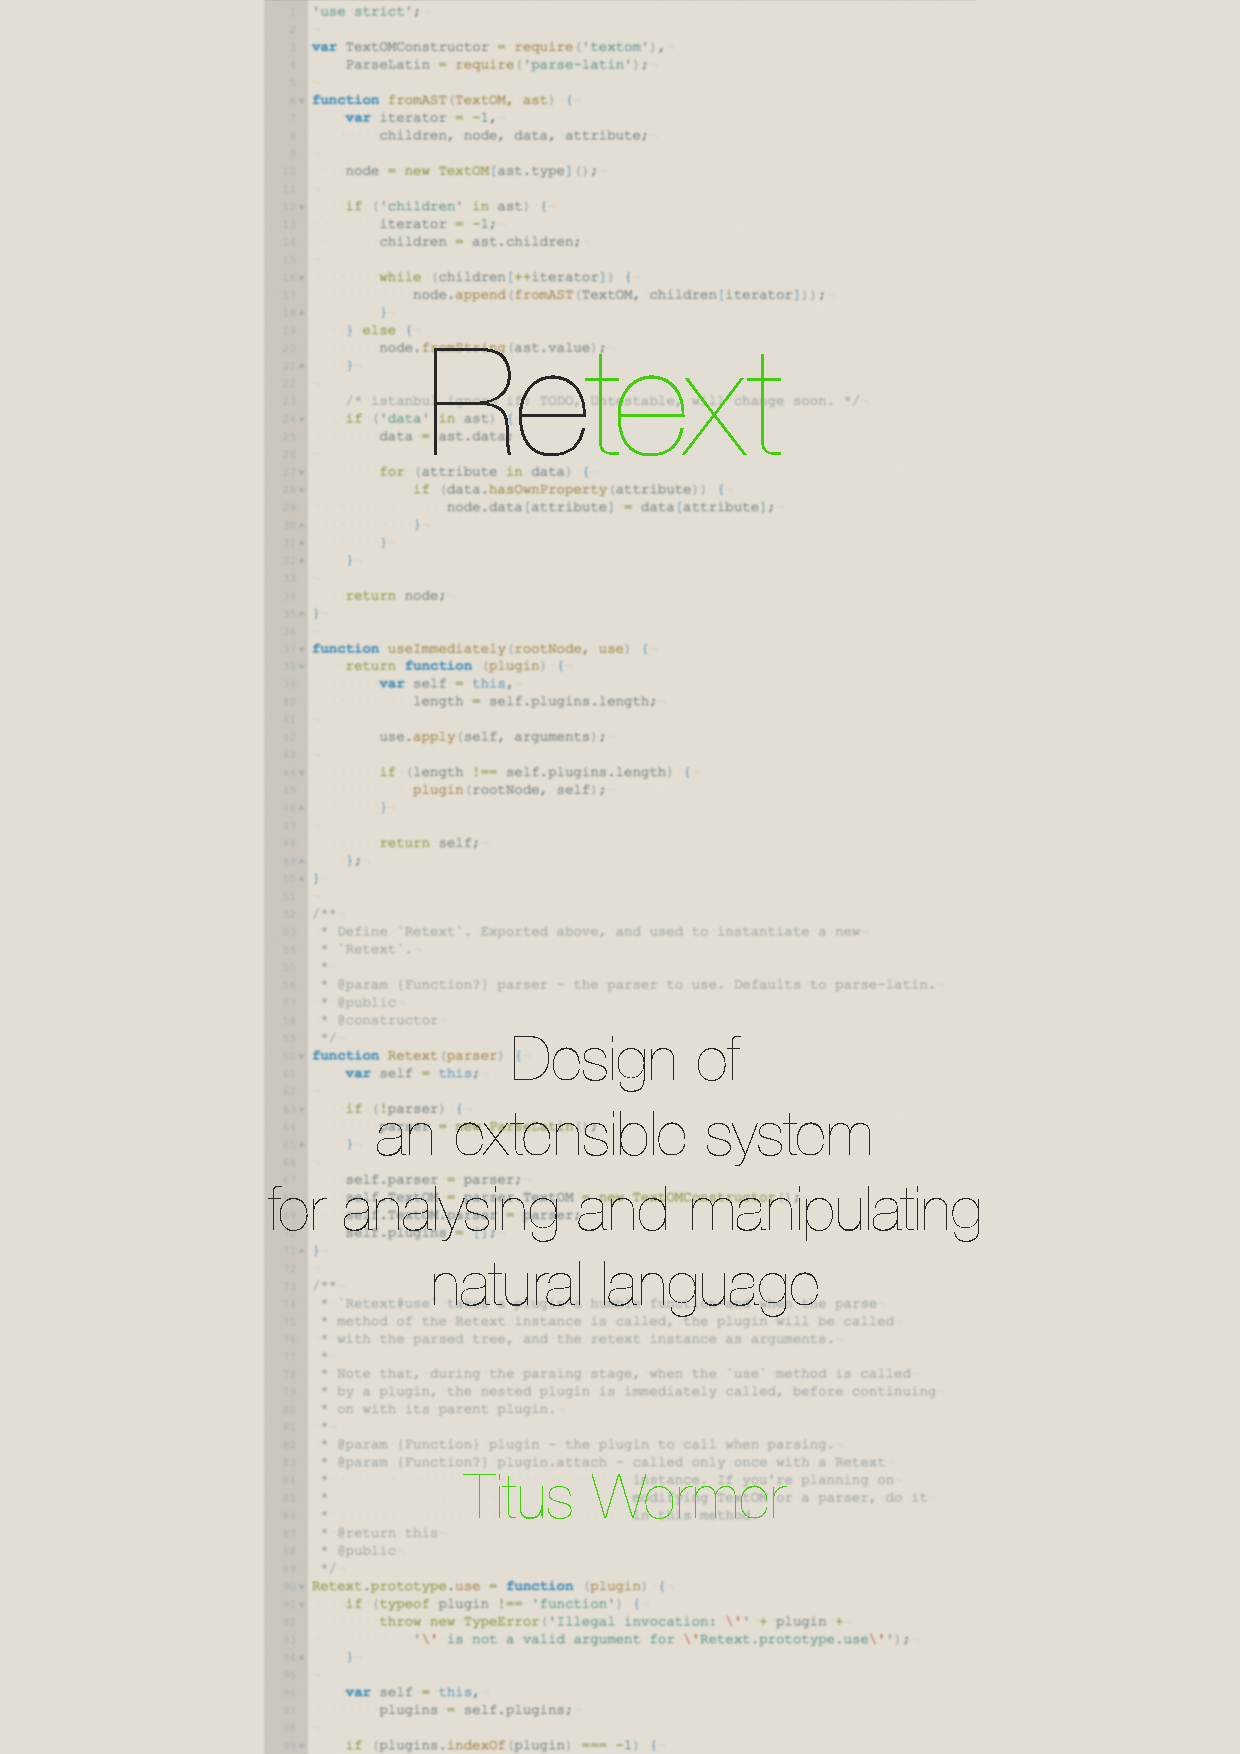
\includepdf[pages={1}]{cover.pdf}
%*******************************************************
% Titlepage
%*******************************************************
\begin{titlepage}
	% if you want the titlepage to be centered, uncomment and fine-tune the line below (KOMA classes environment)
	\begin{addmargin}[-1cm]{-3cm}
    \begin{center}
        \large  

        \hfill

        \vfill

        \begingroup
            \color{Maroon}\spacedallcaps{\myTitle} \\ \bigskip
        \endgroup

        \spacedlowsmallcaps{\myName}

        \vfill

        \mySubtitle \\ \medskip   
        %\myDegree \\
        %\myDepartment \\                            
        %\myFaculty \\
        %\myUni \\ \bigskip

        \myTime\ -- \myVersion

        \vfill                      

    \end{center}  
  \end{addmargin}       
\end{titlepage}   
\thispagestyle{empty}

\hfill

\vfill

\noindent\myName: \textit{\myTitle,} \mySubtitle, %\myDegree, 
\textcopyright\ \myTime

%\bigskip
%
%\noindent\spacedlowsmallcaps{Supervisors}: \\
%\myProf \\
%\myOtherProf \\ 
%\mySupervisor
%
%\medskip
%
%\noindent\spacedlowsmallcaps{Location}: \\
%\myLocation
%
%\medskip
%
%\noindent\spacedlowsmallcaps{Time Frame}: \\
%\myTime

\cleardoublepage%*******************************************************
% Acknowledgments
%*******************************************************
\pdfbookmark[1]{Acknowledgments}{acknowledgments}

\begingroup
\let\clearpage\relax
\let\cleardoublepage\relax
\let\cleardoublepage\relax
\chapter*{Acknowledgments}

Thanks to my supervisor Justus for the trust in me and my work, and for
allowing me to produce a product and thesis that perhaps not every CMD
professional understands, but most certainly falls within our field.

\endgroup

\cleardoublepage%*******************************************************
% Abstract
%*******************************************************
% to have the abstract a bit from the rest in the toc
\refstepcounter{dummy}
\addtocontents{toc}{\protect\vspace{\beforebibskip}}
\addcontentsline{toc}{chapter}{\tocEntry{Abstract}}

\begingroup
\let\clearpage\relax
\let\cleardoublepage\relax
\let\cleardoublepage\relax

\chapter*{Abstract}

This document captures the use cases and requirements for designing and
standardising a solution for textual manipulation and analysis in
\gls{ecmascript}. In addition, this paper presents an implementation that
meets these requirements and answers these use cases.

\endgroup


\cleardoublepage%*******************************************************
% Executive Summary
%*******************************************************
% to have the executive summary a bit from the rest in the toc
\refstepcounter{dummy}
\addtocontents{toc}{\protect\vspace{\beforebibskip}}
\addcontentsline{toc}{chapter}{\tocEntry{Executive Summary}}

\begingroup
\let\clearpage\relax
\let\cleardoublepage\relax
\let\cleardoublepage\relax

\chapter*{Executive Summary}

\gls{nlp} covers many different tasks, but the process of accomplishing
  these goals touches on well defined stages
  (§ \ref{natural-language-processing},
  p. \pageref{natural-language-processing}).
Such as \emph{tokenisation}, the main focus of the proposal.
Current implementations on the web platform are lacking
  (§ \ref{implementations}, p. \pageref{implementations}).
In part, because advanced machine learning techniques (such as
  \emph{supervised learning}) do not work on the web
  (§ \ref{using-corpora-for}, p. \pageref{using-corpora-for}).

The audience that benefits the most from better parsing on the web platform,
  are web developers, a group which is more interested in practical use, and
  less so in theoretical applications
  (§ \ref{target-audience}, p. \pageref{target-audience}).

The target audiences use cases for \gls{nlp} on the web are vast. Examples
  include automatic summarisation, sentiment recognition, spam detection,
  typographic enhancements, counting words, language recognition, and more
  (§ \ref{use-cases}, p. \pageref{use-cases}).

The presented proposal is split into several smaller solutions.
These solutions come together in a proposal: \emph{Retext}, a complete
  natural language system (§ \ref{design}, p. \pageref{design}).
\emph{Retext} takes care of parsing natural language and enables users to
  create and use plugins (§ \ref{natural-language-system-retext},
  p. \pageref{natural-language-system-retext}).

Parsing is delegated to \emph{parse-latin} and others, which first tokenise
  text into a list of words, punctuation, and white space. Later, these
  tokens are parsed into a syntax tree, containing paragraphs, sentences,
  embedded content, and more. Their intelect extends several well known
  techniques (§ \ref{parser-parse-latin}, p. \pageref{parser-parse-latin}).

The objects returned by \emph{parse-latin} and others are defined by
  \acrshort{nlcst}. \acrshort{nlcst} defines the syntax for these objects.
  \acrshort{nlcst} is designed in simmilarity to other popular syntax tree
  specifications (§ \ref{syntax}, p. \pageref{syntax}).

The interface to analyse and manipulate these object is implemented by
  \gls{textom}. \gls{textom} is created in similarity to other, for the target
  audience well known, techniques
  (§ \ref{object-model}, p. \pageref{object-model}).

The proposal was validated both by solving the audiences use cases, and
  by measuring the audiences enthusiasm.
The use cases were validated by implementing many as plugins for
  \emph{Retext} (§ \ref{plugins}, p. \pageref{plugins}).
The enthusiasm showed by the target audience on social networks, through
  email, and social coding was positive
  (§ \ref{reception}, p. \pageref{reception}).

\endgroup

\cleardoublepage%*******************************************************
% Abstract
%*******************************************************
% to have the introduction a bit from the rest in the toc
\refstepcounter{dummy}
\addtocontents{toc}{\protect\vspace{\beforebibskip}}
\addcontentsline{toc}{chapter}{\tocEntry{Introduction}}

\begingroup
\let\clearpage\relax
\let\cleardoublepage\relax
\let\cleardoublepage\relax

\chapter*{Introduction}

\Gls{nlp}, a field of computer science, artificial intelligence, and
  linguistics concerned with the interaction between computers and human
  languages, is becoming more important in society.
For\,example, search engines provide answers before being questioned,
  intelligence agencies detect threats of violence in text messages, and
  e-mail applications know if you forgot to include an attachment.

Despite increased interest, web developers trying to solve \gls{nlp} problems
  reinvent the wheel over and over.
There are tools, especially for other platforms---such\,as in Python
  \autocite{nltk-source} and Java \autocite{opennlp-source}---but they either
  take a too na\"ive approach\footnote{Such\,as ignoring white space
    \autocite{loadfive/knwl-source-code}, implementing a na\"ive
    definition of ``words'' \autocite{nhunzaker/speakeasy-source-code},
    or by using an inadequate algorithm to detect sentences
    \autocite[][]{nytimes/emphasis-source-code}.}, or try to do
  everything\footnote{Although a do-all library
    \autocite[such\,as][]{NaturalNode/natural-source-code} works well on
    server side platforms, it fares less well on the web, where modularity
    and moderation
  are in order.}.
What is missing is a standard representation of the grammatical hierarchy
  of text and a standard for multipurpose analysis of natural language.

My initial interest in natural language was sparked by typography, when I
  felt the need to create a typographically beautiful website, somewhere in
  the summer of 2013.
I felt a craving to apply the tried-and-true practices of typography found on
  paper, to the web.
I was inspired by how these practices were available on other platforms,
  on \TeX{} or \LaTeX, with tools such\,as \emph{microtype}
  \autocite{microtype}, and the \emph{ClassicThesis} theme
  \autocite{classicthesis} based on \emph{The Elements of Typographic Style}
  \autocite{bringhurst-element-typographic-style}.

My interest for fixing typography on the web was piqued.
Thus, I began work on \emph{MicroType.js}, an unpublished library, to
  enable several graphic and typographic practices on the web.
Examples include automatic initials, ligatures, optical margin alignment,
  acronym recognition, smart punctuation, automatic hyphenation, character
  transpositions, and more.
The possibilities were vast, but I noticed how the underlying parser and data
  representation were incomplete.
How words, white space, punctuation, and sentences were defined, was not
  good enough.
The website never came into existence, but during this thesis, I could
  finally fix this problem.
While working on this thesis, the specification and the product, I developed
  a well thought out and substantiated solution.

\emph{Retext}---the implementation introduced in this thesis---and other
  projects in the \emph{Retext} family are a new approach to the syntax of
  natural text.
Together they form an extensible system for multipurpose analysis of natural
  language in \gls{ecmascript}.

To reach this goal, I have organised my paper into six\,main chapters.
In the first\,chapter the scope of this paper is defined and current
  implementations are reviewed, what they lack and where they excel.
Subsequently, the second\,chapter state a research objective and drafts
  research questions.
The third\,chapter defines conditions for such a proposal, where I touch
  upon the target audience, use cases, and requirements.
In the fourth\,chapter, a better implementation is proposed and its
  architectural design is showed.

The fifth\,chapter describes the steps taken to validate the proposal.
I conclude with a sixth\,chapter that offers information on expanding the
  proposal.

\endgroup

\cleardoublepage%*******************************************************
% Table of Contents
%*******************************************************
%\phantomsection
\refstepcounter{dummy}
\pdfbookmark[1]{\contentsname}{tableofcontents}

% 2 includes up to subsections in the ToC
\setcounter{tocdepth}{2}

% 3 numbers up to subsubsections
\setcounter{secnumdepth}{3}
\manualmark
\markboth{\spacedlowsmallcaps{\contentsname}}{\spacedlowsmallcaps{\contentsname}}

\tableofcontents

\automark[section,subsection,subsubsection]{chapter}
\renewcommand{\chaptermark}[1]{\markboth{\spacedlowsmallcaps{#1}}{\spacedlowsmallcaps{#1}}}
\renewcommand{\sectionmark}[1]{\markright{\thesection\enspace\spacedlowsmallcaps{#1}}}


%********************************************************************
% Mainmatter
%********************************************************************
\pagestyle{scrheadings}
\cleardoublepage
\pagenumbering{arabic}
\part{Retext}

% Reset glossary use.
\glsresetall

\chapter{Context}\label{context}

\section{Natural Language Processing}\label{natural-language-processing}

\begin{quote}
  \textit{Natural Language Processing is a theoretically motivated range
    of computational techniques for analyzing and representing
    naturally occurring texts at one or more levels of linguistic
    analysis for the purpose of achieving human-like language processing
    for a range of tasks or applications.
  }

  \medskip
  ---\,Elizabeth\,D.\,Liddy \autocite*{natural-language-processing-liddy-2001}
\end{quote}

\noindent The focus of this paper is \gls{nlp}.
\gls{nlp} concerns itself with enabling machines to understand human
  language.
This makes \gls{nlp} a field related to human--computer interaction.
Human language, a medium which is easy for humans to understand, poses
  problems for machines.
The Georgetown--\gls{ibm} experiment in 1945, one\,of the first\,applications
  of \gls{nlp}, illustrates this difficulty.
During this study in New\,York, scientists demonstrated a
  Russian--English translation system.
The machine translated more than sixty\,sentences from Russian to English.
The experiment was well publicised in the press and resulted in optimism
  among the public.
The public believed machine translation would be a ``solved problem'' within
  three\,to\,five\,years.
Despite promising first\,results, the following ten years were disappointing
  and led to reduced funding \autocite{hutchins-john-georgetown-ibm-system}.

Machine translation is just one\,of many major challenges involved with
  \gls{nlp}.
Other challenges include generating summaries, detecting references to people
  and places, or extracting opinion.
Many programs exist to carry out these and many other \gls{nlp} challenges.
The approach taken to perform these challenges are often similar between
  implementations.
For\,example, entity linking is often implemented as follows
  \autocite[according to][]{stanbol-enhancer-nlp}:

\begin{enumerate}
\item\emph{Language Detection (optional)}\,---\,Based on the language of the
    given text, the algorithms behind the following steps will change.
  Omitted if the implementation supports a single language;
\item\emph{Sentence Tokenisation (optional)}\,---\,Sentence breaking elevates
    performance and heightens accuracy of the following stages, in
    particular \acrshort{pos} tagging;
\item\emph{Word Tokenisation}\,---\,The entities (words) must be free from
  their surroundings;
\item\emph{\gls{pos} Tagging (optional)}\,---\,It is often desired to link
    several nouns or proper nouns.
  Detecting word categories makes this achievable;
\item\emph{Noun Phrase Detection (optional)}\,---\,Although \emph{apple} and
    \emph{juice} could be two\,entities, it is more appropriate to link to
    one\,entity: \emph{apple juice}.
  Detecting noun phrases makes this possible;
\item\emph{Lemmatisation or Stemming (optional)}\,---\,Be it \emph{walk},
    \emph{walked}, or \emph{walking}, all forms of \emph{walk} could link
    to the same entity.
  Detecting either makes this possible;
\item\emph{Entity Linking}\,---\,Linking detected entities to references,
  such\,as an encyclopaedia.
\end{enumerate}

\noindent \gls{nlp} covers many challenges, but the process of accomplishing
  these challenges touches, as seen above, on well-defined stages.

\section{Scope}\label{scope}

Although many \gls{nlp} challenges exist, the standard and the implementation
  this paper proposes will only cover one: \emph{tokenisation}.
Tokenisation, as defined here, includes breaking sentences, words, and
other grammatical units.

Another limitation of the scope of the proposal, is that it focusses on
  syntactic grammatical units.
Thus, semantic units (phrases and clauses) are ignored.

In addition, the paper focusses on written language (text), thus ignoring
  spoken language.

Last, this paper focusses on Latin script languages: written languages
  using an alphabet based on the classical Latin alphabet.

\section{Implementations}\label{implementations}

While researching algorithms to tokenise natural language, few viable
  implementations were found.
Most algorithms look at either sentence- or word tokenisation (rarely both).
This section describes the current implementations, where they excel, and
  what they lack.

\subsection{Stages}\label{stages}

This section delves into how current implementations accomplish tokenisation.

\subsubsection{Sentence Tokenisation}\label{sentence-tokenisation}

Often referred to as sentence boundary disambiguation\footnote{Both
    sentence tokenisation and sentence boundary disambiguation detect
      sentences.
    Sentence boundary disambiguation focusses on the position where
      sentences break (as in, ``One sentence?\textbar{} Two
      sentences.\textbar{}'', where the pipe symbols refer to the end of
      one\,sentence and the beginning of another).
    Sentence tokenisation targets both the start and end positions (as in,
      ``\{One sentence?\} \{Two sentences.\}'', where everything between
      braces is classified as a sentence).}, sentence
  tokenisation is an elementary but important part of \gls{nlp}.
It is almost always a stage in \gls{nlp} applications and not an end goal.
Sentence tokenisation makes other stages (such\,as detecting plagiarism or
  \gls{pos} tagging) perform better.

Often, sentences end in one\,of three\,symbols: either a full stop (.),
  an interrogative point (?), or an exclamation point (!)\footnote{One
    could argue the in 1962 introduced
    obscure interrobang (‽), used to punctuate rhetorical statements where
    neither the question nor exclamation alone exactly serve the writer
    well, should be in this list \autocite{interrobang-mks.com}.}.
But detecting the boundary of a sentence is not as simple as breaking it at
  these markers: they might serve other purposes.
Full stops often occur in numbers, suffixed to abbreviations or titles,
  in initialisms\footnote{Although
    the definition of initialism is ambiguous, this paper defines its use
    as an acronym (an abbreviation formed from initial components, such\,as
    ``sonar'' or ``\textsc{fbi}'') with full stops depicting elision (such\,as
    ``e.g.'', or ``K.G.B.'').},
  or in embedded content\footnote{Embedded
      content in this paper refers to an external (ungrammatical) value
      embedded into a grammatical unit, such\,as a \textsc{url} or an emoticon.
    Note that these embedded values often consist of valid words and
      punctuation marks, but almost always should not be classified as such.}.
Interrogative points as well as exclamation points can occur ambiguously,
  such\,as in a quote (as in `\,``Of course!'', she screamed').

Disambiguation gets even harder when these exceptions \emph{are} in fact a
  sentence boundary (double negative), such\,as in
  ``\ldots{}use the feminine form of idem, ead.'' or in
  `\,``Of course!'', she screamed, ``I'll do it!''\,', where in both
  cases the last terminal marker ends the sentence.

\subsubsection{Word Tokenisation}\label{word-tokenisation}

Like sentence tokenisation, word tokenisation is another elementary but
important stage in \gls{nlp} applications. Whether stemming, finding
phonetics, or \gls{pos} tagging, tokenising words is an important
precursory step.

Often implementations see words as everything that is \emph{not} white
  space (spaces, tabs, feeds) and their boundaries as everything that
  \emph{is} white space \autocite{loadfive/knwl-source-code}.

Some implementations take punctuation marks into account as boundaries.
This practice has flaws, as it results in the faulty classification of
  inner-word punctuation\footnote{Many such inner-word symbols exist,
    such\,as hyphenation points, colons (``12:00''), or elision (whether
    denoted by full stops, ``e.g.''; apostrophes, the Dutch ``'s''; or
    slashes, ``N/A'').}
  as part of the surrounding word \autocite{NaturalNode/natural-source-code}.

\subsection{Challenges}\label{challenges}

The previous section covered implementations that solve tokenisation stages
  in \gls{nlp} applications, such\,as Natural's word
  tokenisers \autocite{NaturalNode/natural-source-code}.
Concluded was that these implementations are lacking.
This section covers several implementations that solve these stages
  as part of a larger challenge.

\subsubsection{Sentiment Analysis}\label{sentiment-analysis}

Sentiment analysis is an \gls{nlp} challenge concerned with the polarity
  (positive, negative) and subjectivity (objective, subjective) of text.
It could be part of an implementation to detect messages with a certain
  polarity.
Twitter allows its users to search on polarity.
For\,example, when a user searches for ``movie :)'', Twitter searches for
  positive tweets.

Sentiment analysis could be implemented as follows:

\begin{enumerate}
\item\emph{Detect Language (optional)};
\item\emph{Sentence Tokenisation (optional)}\,---\,Different sentences have
    different sentiments, tokenising them helps provide better results;
\item\emph{Word Tokenisation}\,---\,Needed to compare with the database;
\item\emph{Lemmatisation or Stemming (optional)}\,---\,Helps classification;
\item\emph{Sentiment Analysis}.
\end{enumerate}

\noindent Sentiment analysers typically include a
  database mapping either words, stems, or lemmas to their respective
  polarity and\slash or subjectivity\footnote{For\,example, the \textsc{afinn}
    database mapping words to polarity \autocite{nielsen-finn-arup-afinn}.}
  and return the average sentiment per sentence, or for the document.

In the case of the previously mentioned Twitter example, the service filters
  out all neutral and negative results, and return the remaining (positive
  attitude) results.

Many implementations exist for this challenge
  \autocites{thinkroth/sentimental-source-code}{mileszim/sediment-source-code}
  {thisandagain/sentiment-source-code}, many of which do not include
  inner-word punctuation in their \emph{definition} of words, resulting in
  less than perfect results\footnote{In fact, all found implementations
      deploy lacking tokenisations steps.
    Dubious, as they each create unreachable code through their na\"ivety:
      all implementations remove dashes from words, while words such\,as
      ``self-deluded'' are included in the databases they use, but never
      reachable.}.

\subsubsection{Automatic Summarisation}\label{automatic-summarisation}

Automatic summarisation is an \gls{nlp} challenge concerned with the reduction
  of text to the \emph{major} points retaining the original document.
Few open source implementations of automatic summarisation algorithms on
  the web, in contrast with implementations for sentimental analysis, were
  found\footnote{For\,example, on the web only \emph{node-summary} was found
    \autocite{jbrooksuk/node-summary-source-code}, in Scala \emph{textteaser}
    was found \autocite{MojoJolo/textteaser-source-code}.}.

Automatic summarisation could be implemented as follows:

\begin{enumerate}
\item\emph{Detect Language (optional)};
\item\emph{Sentence Tokenisation (optional)}\,---\,Unless even finer grained
  control over the document is possible (tokenising phrases), sentences are
  the smallest unit that should stay intact in the resulting summary;
\item\emph{Word Tokenisation}\,---\,Needed to calculate keywords (words
  which occur more often than expected by chance alone);
\item\emph{Automatic Summarisation}.
\end{enumerate}

\noindent Automatic summarisers typically return the highest ranking units,
  be it sentences or phrases, according to several factors:

\begin{aenumerate}
\item\emph{Number of Words}\,---\,An ideal sentence is neither too long nor
  too short;
\item\emph{Number of Keywords}\,---\,Words which occur more often than
  expected by chance alone in the text;
\item\emph{Similarity to Title}\,---\,Number of words from the document's
  title the sentence or phrase contains;
\item\emph{Position Inside Parent}\,---\,Initial and final sentences of a
  paragraph are often more important than sentences buried somewhere in
  the middle.
\end{aenumerate}

\noindent Some implementations include only keyword metrics
  \autocite{jbrooksuk/node-summary-source-code}, others include all features
  \autocite{MojoJolo/textteaser-source-code}, or even more advanced factors
  \autocite{summly}.

The only implementation working on the web, by James\,Brook
  \autocite*{jbrooksuk/node-summary-source-code}, takes a na\"ive sentence
  tokenisation approach, such as ignoring sentences terminated by
  exclamation marks.
Both other implementations, and many more, use a different approach to
  sentence tokenisation: corpora.

\subsection{Using Corpora for \textsc{nlp}}\label{using-corpora-for}

A corpus (plural: corpora) is a large, structured set of texts used for many
  \gls{nlp} and linguistics challenges.
Corpora contain items (often words, but sometimes other units) annotated
  with information (such\,as \gls{pos} tags or lemmas).

These colossal (often more than a million words\footnote{The Brown\,Corpus
    contains about a million words \autocite{francis-nelson-brown-corpus},
    the Google N-Gram\,Corpus contains 155\,billion
    \autocite{brants-thorsten-google-ngram-corpus}.})
  lumps of data are the basis of many of the newer revolutions in \gls{nlp}
  \autocite{mitkov-ruslan-ea-importance-corpora}.
Parsing based on supervised learning (in \gls{nlp}, based on annotated
  corpora), is the opposite of rule based parsing\footnote{A simple
    rule based sentence tokeniser could be implemented as follows
    \autocite{attivio.com-doing-things-with-sentences}:

    \begin{aenumerate}
      \item If it is a full stop, it ends a sentence;
      \item If the full stop is preceded by an abbreviation, it does not end
        a sentence;
      \item If the next token is capitalised, it ends a sentence.
    \end{aenumerate}}.
Instead of rules (and exceptions to these rules, exceptions to these
  exceptions, and so on) specified by a developer,
  supervised learning\footnote{``{[}From{]} a set of labelled examples as
    training data {[}, make{]} predictions for all unseen points''
    \autocite{mohri-mehryar-foundations-machine-learning}.}
  delegates this task to machines.
This delegation results in a more efficient, scalable, program.

Parsing based on corpora has proven better over rule based
  parsing in several ways, but has disadvantages:

\begin{enumerate}
\item Good training sets are required;
\item If the corpus was created from news articles, algorithms based on it
  will not fare so well on microblogs (such\,as Twitter posts).
\item Some rule based approaches for pre- and post processing are still
  required.
\end{enumerate}

\noindent In addition, corpora based parsing will not work well on the web.
Loading corpora over the network each time a user requests a web page is
  infeasible for most websites and applications\footnote{Currently,
      one\,technology exists for storing large datasets in a browser: the
      \acrshort{html5} File System \acrshort{api}.
    However, ``work on this document has been discontinued'', and the
      specification ``should not be used as a basis for implementation''
      \autocite{urhane-file-api}.}.

Two viable alternative approaches exist for the web: rule based tokenisation,
  or connecting to a server over the network.

\subsection{Using a Web \textsc{api}}\label{using-a-web}

Where the term \gls{api} stands for an interface between two\,programs,
  it is often used in web development as requests (from a web browser),
  and responses (from a web server) over \gls{http}.
For\,example, Twitter has such a service to allow developers to list,
  replace, create, and delete so-called tweets and other objects (such\,as
  users or images).
This paper uses the term Web \gls{api} for the latter, and \gls{api} for
any programming interface.

With the rise of the asynchronous web\footnote{Around 2000,
    \gls{ajax} started to transform the web.
  Before, significant changes to websites only occurred when a user
    navigated to a new page. 
  With \gls{ajax} however, new content arrived to users without the need
    for a full page refresh.
  The first\,examples of how \gls{ajax} made the web feel more like native
    applications, are Outlook Web Access in 2000
    \autocite{technet-outlook-web-access} and Gmail in 2004
    \autocite{gmailblog-gmail-ajax}.},
  supervised learning became available through web \glspl{api}
  \autocites{textteaser-web-api}{wordnet-web-api}{textrazor-web-api}.
This made it possible to use supervised learning techniques on the web,
  without needing to download corpora to a users' computer.

However, accessing \gls{nlp} web \glspl{api} over a network has
  disadvantages.
Foremost of which the time involved in sending data over a network and
  bandwidth used (especially on mobile networks), and heightened security
  risks.

\chapter{Research Framework}\label{research-framework}

This chapter states the objective of this paper (§~\ref{research-objective}).
From the objective a research question is drafted (§~\ref{research-question}).
Additionally, from the research question, several research questions are
  drafted, acting as a guideline for the proposal
  (§~\ref{research-questions}).

\section{Research Objective}\label{research-objective}

Using the context described in chapter \ref{context} (p.~\pageref{context}),
  the objective of this research project is constructed:

\begin{quote}
  \textit{A generic documentation (the ``specification'') and example
    implementation (the ``program'') that exposes an interface (the
    ``\acrshort{api}'') for the topic (``text manipulation'') based on real
    use cases of potential users (the ``developer'') on the platform (the
    ``web'').
  }
\end{quote}

\section{Research Question}\label{research-question}

This research objective leads to a research question:

\begin{quote}
  \textit{How can a specification and program, that exposes an \acrshort{api}
    for text manipulation, based on use cases of developers on the web,
    be developed?
  }
\end{quote}

\section{Research Questions}\label{research-questions}

The previously defined research question is split into several smaller
  questions.
These research questions form a basis and a guide to answer the research
  question, to reach the research objective.

\begin{enumerate}
\item
  What are current possibilities and deficiencies in \gls{nlp}?
  \begin{enumerate}
    \item What current implementations exist?
    \item What does not yet exist?
  \end{enumerate}
\item
  How to ensure a quality implementation for the target audience?
  \begin{enumerate}
    \item What makes a good \gls{api} design?
    \item What makes a good implementation?
  \end{enumerate}
\item
  What are the target audience's use cases for an implementation?
  \begin{enumerate}
    \item What would they use an implementation for?
    \item What would they \emph{not} use the implementation for?
  \end{enumerate}
\end{enumerate}

\chapter{Production}\label{production}

\section{Target Audience}\label{target-audience}

The audience that benefits the most from the proposal (the reached research
  objective, \emph{Retext}), are web developers.
Web developers are programmers who specialise in creating software that
  functions on the world wide web.
A group which enables machines to respond to humans.
They engage in client side development (building the interface between
  a human and a machine on the web), and sometimes also in server side
  development (building the interface between the client side and a
  server).

Typical areas of work consist of programming in \gls{ecmascript},
  marking up documents in \gls{html}, graphic design through \gls{css},
  creating a back end in Node.js, \gls{php}, or other platforms, contacting a
  \gls{mongodb}, \gls{mysql}, or other database, and more.

Additionally, many interdisciplinary skills, such as usability,
  accessibility, copywriting, information architecture, or optimisation,
  are also of concern to web developers.

\section{Use Cases}\label{use-cases}

There are many use cases of the target audience, the web developer, in the
  field of \gls{nlp}.
Research for this paper found several use cases, although it is
  expected many more could be defined.
The use cases below are annotated with broad, generic categories:
  analysation, manipulation, and creation.

\begin{aenumerate}
\item\label{list:use-case:1} The developer may intent to summarise natural
  text (mostly analysation, potentially also manipulation);
\item\label{list:use-case:2} The developer may intent to create natural
  language, such as displaying the number of unread messages: ``You have 1
  unread message'', or ``You have 0 unread messages'' (creation);
\item\label{list:use-case:3} The developer may intent to recognise sentiment
  in text: is a \emph{tweet} positive, negative, or spam? (analysation);
\item\label{list:use-case:4} The developer may intent to replace so-called
  \emph{dumb} punctuation with \emph{smart} punctuation, such as dumb
  quotations with (``) or (''), three\,dots with an ellipsis (\ldots{}), or
  two\,hyphens with an en-dash (--) (manipulation);
\item\label{list:use-case:5} The developer may intent to count the number of
  certain grammatical units in a document, such as words, white space,
  punctuation, sentences, or paragraphs (analysation);
\item\label{list:use-case:6} The developer may intent to recognise the
  language in which a document is written (analysation);
\item\label{list:use-case:7} The developer may intent to find words in a
  document based on a search term, with regards to the lemma (or stem)
  and\slash or phonetics (so that a search for ``smit'' also returns similar
  words, such as ``schmidt'' or ``Smith'') (analysation and manipulation).
\end{aenumerate}

\noindent \gls{nlp} is a large field with many challenges, but not every
  challenge in the field is of interest to the web developer.
Foremost, the more academic areas of \gls{nlp}, such as speech recognition,
  optical character recognition, text to speech transformation, translation,
  and machine learning, do not fit well within the goals of web developers.

\section{Requirements}\label{requirements}

The proposal must enable the target audience to reach the in the previous
  section defined use cases.
In addition, the proposal should meet several other requirements to better
  suit the wishes of the target audience.

\subsection{Open Source}\label{open-source}

To reach the target audience and validate its usability, the proposal
  should be open source.
All code should be licensed under \acrshort{mit}, a license which
  provides rights for others to use, copy, modify, merge, publish,
  distribute, sublicense, and\slash or sell copies of the code it covers.

In addition, the software should be developed under the all-seeing eye of
  the community: on GitHub.
GitHub is a hosted version control\footnote{Version
    control services manage revisions to documents, popularly used for
    controlling and tracking changes in software.} service with social
  networking features.
On GitHub, web developers follow their peers to track what they are
  working on, watch their favourite projects to get notified of changes,
  and raise issues and request features.

\subsection{Performance}\label{performance}

The proposal should be executed at high \emph{performance}.
Performance includes the software having a small file size to reach the
  client over the network with the highest possible speed.
But most importantly, the execution of code should run efficiently and
  at high speeds.

\subsection{Testing}\label{testing}

\emph{Testing} should have high priority in the proposal.
Testing, in software development, refers to validating if software does what
  it is supposed to do, and can be divided into several subgroups:

\begin{aenumerate}
\item\emph{Unit Testing}\,---\,Each specific section of code;
\item\emph{Integration Testing}\,---\,How programs work together;
\item\emph{System Testing}\,---\,If the system meets its
  requirements;
\item\emph{Acceptance Testing}\,---\,The end product.
\end{aenumerate}

\noindent Great care should be given to develop an adequate test suite with
  full \emph{coverage} for every program.
Coverage, in software development, is a term used to describe the amount of
  code tested by the test suite.
Full coverage means every part of the code is reached by the tests.

Unit test run through Mocha \autocite{visionmedia/mocha-source-code},
  coverage is detected by Istanbul
  \autocite{gotwarlost/istanbul-source-code}.

\subsection{Code Quality}\label{code-quality}

\emph{Code quality}---how useful and readable for both humans and machines
  the software is---should be vital.
For humans, the code should be consistent and clear.
For computers, the code should be free of bugs and other suspicious code.

\subsubsection{Suspicious Code \& Bugs}\label{suspicious-code-and-bugs}

To detect bugs and suspicious code in the software, \emph{Eslint}
  is used \autocite{eslint/eslint-source-code}.
\emph{Linting}, in computer programming, is a term used to describe static
  code analysis to detect syntactic discrepancies without running the code.
\emph{Eslint} is used because it provides a solid set of basic rules and
  enables developers to create custom rules.

\subsubsection{Style}\label{style}

To enforce a consistent code style---to create readable software for
  humans---\acrshort{jscs} is used \autocite{mdevils/node-jscs-source-code}.
\acrshort{jscs} provides rules for (dis)allowing certain code patterns,
  such as white space at the end of a line or camel cased variable names,
  or enforcing a maximum line length.
\acrshort{jscs} was chosen because it, like \emph{Eslint}, provides a strong
  basic set of rules.
The rules chosen for the proposal were set strict to enforce all code to be
  written in the same way.

\subsubsection{Commenting}\label{commenting}

Even when code is bug free, uses no confusing short-cuts, and adheres to a
  strict style, it might still be hard to understand for humans.
\emph{Commenting} code---describing what a program does and why it
  accomplishes it this way---is important.
However, commenting can also be too verbose, such as when the code is
  duplicated in natural language.

\gls{jsdoc} \autocite{google.com-clojure-compiler-jsdoc} is a markup language
  for \gls{ecmascript} that allows developers to embed documentation---using
  comments---in source code.
Several tools can later extract this information and expose it independent
  from the original code.
``Tricky'' code should be annotated inside the software with comments to help
  readers understand why certain decisions were made.

\subsection{Automation}\label{automation}

When suspicious, ambiguous, or buggy code is introduced in the software, the
  error should be automatically detected.
Sometimes, deployment should be prevented.
Automated \gls{ci} environments to enforce error detection should be used.
To detect complex, duplicate, or bug prone code, Code\,Climate is used
  \autocite{codeclimate.com}.
To validate all tests passed before deploying the software, Travis is used
  \autocite{travis-ci.org}.

\subsection{\textsc{api} Design}\label{design-1}

Quality interface design should have high priority for the proposal.
A good \gls{api}, according to Joshua\,Bloch
  \autocite*{bloch-joshua-how-design-good-api-why-matters}, has the following
  characteristics:

\begin{enumerate}
\item Easy to learn;
\item Easy to use;
\item Hard to misuse;
\item Easy to read;
\item Easy to maintain;
\item Easy to extend;
\item Meeting its requirements;
\item Appropriate for the target audience.
\end{enumerate}

\noindent In essence equal, but worded differently, are the characteristics
  of good \gls{api} design according to the Qt\,Project
  \autocite*{qt-project.org-api-design-principles}:

\begin{enumerate}
\item Be minimal;
\item Be complete;
\item Have clear and simple semantics;
\item Be intuitive;
\item Be easy to memorise;
\item Lead to readable code.
\end{enumerate}

\noindent The proposal should take these characteristics, and their given
  examples, into account.

\subsection{Installation}\label{installation}

Simple access to the software for the target audience, both on the client
  side and on the server side, should be given high priority.
On the client side, many package managers exist, the most
  popular being Bower and Component\footnote{Popularity here is simply
    defined as having the highest number of search results on Google.}.
For Node.js (on the server side), \gls{npm} is the most popular.
To reach the target audience, besides making the source available on GitHub,
  all popular package managers, \gls{npm}, Bower, and Component, are used.

\chapter{Design \& Architecture}\label{design}

The in this paper presented solution to the problem of \gls{nlp} on the
  client side is split up in multiple small proposals.
Each sub-proposal solves a sub-problem.

\begin{aenumerate}
\item\acrshort{nlcst} defines a standard for classifying grammatical units,
  understandable for machines;
\item\emph{parse-latin} classifies natural language according to
  \acrshort{nlcst};
\item\gls{textom} provides an interface for analysing and manipulating output
  provided by \emph{parse-latin};
\item\emph{Retext} provides an interface for transforming natural language
  into an object model and exposes an interface for plug-ins.
\end{aenumerate}

\noindent The decoupled approach taken by the provided solution enables other
  developers to implement their own software to replace sub-proposals.
For example, other parties could create a parser for the Chinese language and
  use it instead of \emph{parse-latin} to classify natural language according
  to \gls{nlcst}, or other parties can implement an interface like
  \gls{textom} with functionality for phrases and clauses.

\section{Syntax: \textsc{nlcst}}\label{syntax}

To develop natural language tools in \gls{ecmascript}, an intermediate
  representation of natural language is useful.
Instead of each module (such\,as every stage in section
  \ref{sentiment-analysis} on page\,\pageref{sentiment-analysis})
  defining its own representation of text, using a single syntax leads to
  better interoperability, performance, and results.

The elements defined by \acrfull{nlcst} are based on the grammatical
  hierarchy, but by default do not expose all its constituents\footnote{The
      grammatical hierarchy of text is constituted by words, phrases,
      clauses, and sentences.
    \glspl{nlcst} only implements the sentence and word constituents
    by default, although clauses and phrases could be provided by
    implementations.}.
Additionally, \gls{nlcst} provides elements to cover other semantic units in
  natural language\footnote{Most
    notably punctuation, embedded content, and white space elements.}.

The definitions were influenced by other syntax trees specifications for
  manipulation on the web platform, such\,as \emph{\textsc{css}}, eponymous
  for the \acrshort{css} language \autocite{reworkcss/css-source-code} or the
  \emph{Mozilla JavaScript \textsc{ast}}, for \gls{ecmascript}
  \autocite{mozilla.org-spidermonkey-parser_api}.

Both widely used implementations, \emph{\textsc{css}} by \emph{Rework}
  \autocite{reworkcss/rework-source-code}, and \emph{Mozilla JavaScript
  \textsc{ast}} by \emph{Esprima} \autocite{ariya/esprima-source-code},
  \emph{Acorn} \autocite{marijnh/acorn-source-code}, and \emph{Escodegen}
  \autocite{constellation/escodegen-source-code}.

\gls{nlcst} differs from both specifications by implementing a \gls{cst},
  where the others use an \gls{ast}.
A \gls{cst} is a one-to-one\,mapping of source (such\,as natural language)
  to result (a tree).
All information stored in the source is also available through the tree
  \autocite{thegreenplace.net-abstract-concrete-syntax-trees}.
This makes it easy for developers to save the output or pass it on to other
  libraries for further processing.
However, the information stored in \glspl{cst} is verbose, which might be
  difficult to work with.

\medskip\noindent See appendix\,\ref{appendix-nlcst} on
  page\,\pageref{appendix-nlcst} for a list of specified nodes of \gls{nlcst}.

\section{Parser: \emph{parse-latin}}\label{parser-parse-latin}

To create a syntax tree according to \gls{nlcst} from natural language,
  this paper presents \emph{parse-latin} for Latin script based
  languages\footnote{Such\,as Old-English, Icelandic, French, or even scripts
    slightly similar, such\,as Cyrillic, Georgian, or Armenian.}.
Additionally, to prove the concept, two\,other libraries are presented,
  \emph{parse-english} and \emph{parse-dutch}.
Both with \emph{parse-latin} as a basis, but providing better support for
  several language specific features, respectively for English and Dutch.

By using the \gls{cst} as described by \gls{nlcst} and the \emph{parse-latin}
  parser, the intermediate representation can be used by developers to
  create independent modules which may receive better results or
  performance over implementing their own parsing tools.

In essence, \emph{parse-latin} tokenises text into white space, word, and
  punctuation tokens.
\emph{parse-latin} starts out with a pretty simple definition, one that
  some other tokenisers also implement \autocite{treebank-tokenisation}:

\begin{enumerate}
\item A \emph{word} is one\,or more\,letter or number characters;
\item A \emph{white space} is one\,or more\,white space characters;
\item A \emph{punctuation} is one\,or more\,of anything else.
\end{enumerate}

\noindent Then, \emph{parse-latin} manipulates and merges those tokens into a
  syntax tree, adding sentences, paragraphs, and other nodes where needed.
Most of the intellect of the algorithm deals with sentence tokenisation
  (§\,\ref{sentence-tokenisation}, p.\,\pageref{sentence-tokenisation}).
This is done in similar fashion, but more intelligent, to \emph{Emphasis}
  \autocite{nytimes/emphasis-source-code}.

\begin{aenumerate}
\item\emph{Inter-word Punctuation}\,---\,Some punctuation marks are part of
  the word they occur in, such\,as the punctuation marks in ``non-profit'',
  ``she's'', ``G.I.'', ``11:00'', or ``N\slash A'';
\item\emph{Non-terminal Full Stops}\,---\,Some full stops do not mark a
  sentence end, such\,as the full stops in ``1.'', ``e.g.'', or ``id.'';
\item\emph{Terminal Punctuation}\,---\,Although full stops, question marks,
  and exclamation marks (sometimes) end a sentence, that end might not occur
  directly after the mark, such\,as the punctuation marks after the full
  stop in ``.)'' or ``.'{}'';
\item\emph{Embedded Content}\,---\,Punctuation marks are sometimes used in
  non-standard ways, such\,as when a section or chapter delimiter is
  created with a line containing three\,asterisk marks (``* * *'').
\end{aenumerate}

\noindent See appendix\,\ref{appendix-parse-latin} on
page\,\pageref{appendix-parse-latin} for example output provided
by \emph{parse-latin}.

\subsection{\emph{parse-english}}\label{parse-english}

\emph{parse-english} provides the same interface as \emph{parse-latin}, but
  returns results better suited for English text.
Exceptions in the English language include:

\begin{aenumerate}
\item \emph{Unit Abbreviations}\,---\,``tsp.'', ``tbsp.'', ``oz.'', ``ft.'',
  etc.;
\item\emph{Time References}\,---\,``sec.'', ``min.'', ``tues.'', ``thu.'',
  ``feb.'', etc.;
\item\emph{Business Abbreviations}\,---\,``Inc.'' and ``Ltd.''
\item\emph{Social Titles}\,---\,``Mr.'', ``Mmes.'', ``Sr.'', etc.;
\item\emph{Rank \& Academic Titles}\,---\,``Dr.'', ``Gen.'', ``Prof.'',
  ``Pres.'', etc.;
\item\emph{Geographical Abbreviations}\,---\,``Ave.'', ``Blvd.'', ``Ft.'',
  ``Hwy.'', etc.;
\item\emph{American State Abbreviations}\,---\,``Ala.'', ``Minn.'', ``La.'',
  ``Tex.'', etc.;
\item\emph{Canadian Province Abbreviations}\,---\,``Alta.'', ``Qué.'',
  ``Yuk.'', etc.;
\item\emph{English County Abbreviations}\,---\,``Beds.'', ``Leics.'',
  ``Shrops.'', etc.;
\item\emph{Elision (omission of letters)}\,---\,``'n'\,'', ``'o'', ``'em'',
  ``'twas'', ``'80s'', etc.
\end{aenumerate}

\subsection{\emph{parse-dutch}}\label{parse-dutch}

\emph{parse-dutch} has, like \emph{parse-english}, the same interface as
  \emph{parse-latin}, but returns results better suited for Dutch text.
Exceptions in the Dutch language include:

\begin{aenumerate}
\item\emph{Unit \& Time Abbreviations}\,---\,``gr.'', ``sec.'', ``min.'', ``ma.'',
  ``vr.'', ``vrij.'', ``febr'', ``mrt'', etc.;
\item\emph{Many Other Common Abbreviations}\,---\,``Mr.'', ``Mv.'', ``Sr.'',
  ``Em.'', ``bijv.'', ``zgn.'', ``amb.'', etc.;
\item\emph{Elision (omission of letters)}\,---\,``d'\,'', ``'n'', ``'ns'',
  ``'t'', ``'s'', ``'er'', ``'em'', ``'ie'', etc.
\end{aenumerate}

\section{Object Model: Text\textsc{om}}\label{object-model}

To modify an \gls{nlcst} tree in \gls{ecmascript}, whether created by
  \emph{parse-latin}, \emph{parse-english}, \emph{parse-dutch}, or other
  parsers, this paper presents \gls{textom}.
\gls{textom} implements the nodes defined by \gls{nlcst},
  but provides an object-oriented style\footnote{Object-oriented
    programming is a style of programming, where classes, instances,
    attributes, and methods are important.} to manipulate these nodes.
\gls{textom} was designed in similarity to the \gls{dom}\footnote{See
    appendix\,\ref{appendix-dom} on page\,\pageref{appendix-dom} for more
    information on the \gls{dom}.},
  the mechanism used by browsers to expose \gls{html} through
  \gls{ecmascript} to developers.
Because of \glspl{textom} likeness to the \gls{dom}, \gls{textom} is
  easy to learn and familiar to the target audience.

\gls{textom} provides functionality for events (a mechanism for detecting
  changes), modification (inserting, removing, and replacing children
  into\slash from parents), and traversal (such\,as finding all words in a
  sentence).

\gls{nlcst} allows authors to extend the specification by defining their
  own units, such\,as creating phrase or clause nodes.
\gls{textom} allows for the same extension, and is built to work well
  with these ``unknown'' nodes.

\medskip \noindent See appendix\,\ref{appendix-textom} on
  page\,\pageref{appendix-textom} for the implementation details of
  \gls{textom}.

\section{Natural Language System:
  Retext}\label{natural-language-system-retext}

For natural language processing on the client side, this paper presents
  \emph{Retext}.
\emph{Retext} combines a parser, such\,as \emph{parse-latin} or
  \emph{parse-english}, with an object model: \gls{textom}.
Additionally, \emph{Retext} provides a minimalistic plug-in mechanism which
  enables developers to create and publish plug-ins for others to use, and in
  turn enables them to use others' plug-ins inside their projects.

\emph{Retext} provides a strong basis to use plug-ins to add simple natural
  language features to a website, but additionally provides functionality to
  extend this basis---create plug-ins, parsers, or other features---to
  create vast natural language systems.

\medskip \noindent See appendix\,\ref{appendix-retext} on
  page\,\pageref{appendix-retext} for a description of the interface
  provided by \emph{Retext} and example usage.

\chapter{Validation}\label{validation}

The presented proposal was validated through two approaches.
The design and the usability of the interface was validated through
  solving several use cases of the target audience with the proposal.
Interest in the proposal by the target audience was validated by
  measuring the enthusiasm showed by the open source community.

\section{Plugins}\label{plugins}

More than fifteen plug-ins for \emph{Retext} were created to confirm if,
  and validate how, the proposals integrated together, and how the system
  worked.

The proposal solves the creation of natural language by default (use case
  \ref{list:use-case:2}), but these plug-ins solve several others.
The developed plug-ins included implementations for:

\begin{aenumerate}
\item Transforming so-called dumb punctuation marks into more
  typographically correct punctuation marks, solving use case
  \ref{list:use-case:4} \autocite*{wooorm/retext-smartypants-source-code};
\item Transforming emoji short-codes (:cat:) into real emoji
  \autocite*{wooorm/retext-emoji-source-code};
\item Detecting the direction of text
  \autocite*{wooorm/retext-directionality-source-code};
\item Detecting phonetics
  \autocite*{wooorm/retext-double-metaphone-source-code};
\item Detecting the stem of words
  \autocite*{wooorm/retext-porter-stemmer-source-code};
\item Finding grammatical units, solving use case
  \ref{list:use-case:5}  \autocite*{wooorm/retext-visit-source-code};
\item Finding text, even misspelled, solving use case
  \ref{list:use-case:7} \autocite*{wooorm/retext-search-source-code};
\item Detecting \gls{pos} tags \autocite*{wooorm/retext-pos-source-code};
\item Finding keywords and -phrases
  \autocite*{wooorm/retext-keywords-source-code};
\item Detecting the language of text, solving use case \ref{list:use-case:6} 
  \autocite*{wooorm/retext-language-source-code}.
\end{aenumerate}

\noindent These plug-ins listed and the other plug-ins solve several use cases
  of the target audience (§~\ref{use-cases}).
The unsolved use cases can be solved using the plug-in mechanism provided by
  \emph{Retext}.
Summarising natural language (use case \ref{list:use-case:1}) is not yet
  solved, but can be by implementing the stages mentioned in
  §~\ref{automatic-summarisation} (p.~\pageref{automatic-summarisation}).
Neither is detecting sentiment (use case \ref{list:use-case:3}), but can be
  by implementing the stages mentioned in §~\ref{sentiment-analysis}
  (p.~\pageref{sentiment-analysis}).

During the development of these plug-ins, several problems were brought to
  light in the developed software.
These problems were recursively dealt with, back and forth, between the
  software and the plug-ins.
The software changed severely by these changes, which resulted in a
  better interface and usability.

\section{Reception}\label{reception}

To confirm interest by the target audience in the proposal, enthusiasm
  showed by the open source community was measured.
To initially spark interest, several websites and e-mail newsletters were
  contacted to feature \emph{Retext}, either in the form of an article or as
  a simple link.
This resulted in coverage on high-profile websites
  \autocite{dailyjs.com-natural-language-parsing-retext} and newsletters
  \autocites{nodeweekly.com-47}{javascriptweekly.com-193}
  {newspaper.io/javascript-2014-08-11}.
Later, organic growth resulted in features on link roundups
  \autocites{github.com-awesome-machine-learning}{github.com-awesome-nodejs},
  Reddit \autocites{reddit.com-mention-1}{reddit.com-mention-2}
  {reddit.com-mention-3}.

In turn, these publications resulted in positive reactions, such as on
  Twitter \autocites{twitter.com-mention-1}{twitter.com-mention-2}
  {twitter.com-mention-3}{twitter.com-mention-4}{twitter.com-mention-5}
  {twitter.com-mention-6}, other websites, and both feedback and fixes
  on GitHub \autocites{github.com-issue-1}{github.com-issue-2}
  {github.com-issue-3}{github.com-pull-request}.

Additionally, many of the target audience started \emph{following} the
  project on GitHub \autocite{github.com-stargazers}.

\chapter{Conclusion}\label{conclusion}

This chapter\,consists of a\,short summary (§\,\ref{summary}), a\,list of
  limitations and suggestions for future work
  (§\,\ref{limitations-future-work}), and a\,list of conclusions
  (§\,\ref{conclusions}).

\section{Summary}\label{summary}

\gls{nlp} covers many challenges.
The process of accomplishing these challenges touches on well-defined stages.
Such\,as \emph{tokenisation}, the focus of this paper.
Current implementations on the web platform are lacking.
In part, because techniques such\,as \emph{supervised learning} do not work
  on the web.

The audience that benefits the most from better parsing on the web platform,
  are web developers, a\,group which is more interested in practical use, and
  less so in theoretical applications.

The presented proposal is split-up in several solutions: a specification,
  a\,parser, and an\,object model.
These solutions come together in a\,proposal: \emph{Retext}, a\,complete
  natural language system.
\emph{Retext} takes care of parsing natural language and enables users to
  create and use plug-ins.

The proposal was validated both by solving the audience's use cases with
  \emph{Retext}, and by measuring the audience's enthusiasm for \emph{Retext}.

\section{Limitations \& Future Work}\label{limitations-future-work}

The proposal leaves open many areas of interest for future investigation.
Some of which are featured here.

\begin{aenumerate}
\item\emph{Internationalisation}\,---\,Currently, the proposal is only
    tested on Latin script languages.
  The software was developed with other languages and scripts, such\,as
    Arabic, Hangul, Hebrew, and Kanji, in mind.
  Future work could expand support to include these scripts;
\item\emph{Difference Application}\,---\,Currently, the proposal does not
    support difference application.
  When a\,word is added at the end of a\,sentence, all steps to produce the
    output have to be revisited.
  Although the proposal is created with this in mind, no support has been
    added.
  Future work could include difference application support;
\item\emph{Non-rule Based Parsing}\,---\,Currently, \gls{nlcst} trees are
    created with rule based parsers.
  But, corpora based parsers could also produce these trees.
  Future work could investigate and implement such supervised learning
    approaches.
\item\emph{Academic Goals}\,---\,Currently, the proposals cater to practical use
    cases.
  Future work could expand on this purview and implement more academic
    goals.
\item\emph{Semantic Units}\,---\,Currently, the proposals provide syntactic
    units.
  Future work could expand on this by providing information about phrases
    and clauses to users.
\item\emph{Source Formats}\,---\,Currently, the parsers each require plain
    text input.
  Future work could expand on this by allowing other input formats, such\,as
    MarkDown or \TeX.
\item\emph{Heighten Performance}\,---\,The decision made to adopt
    an\,object-oriented approach for analysation and manipulation, came at
    a\,huge performance cut.
  When implementing both \gls{textom} and \emph{parse-latin} over just
    \emph{parse-latin}, performance decreases over 90\%.
  Future work should investigate and implement better performance.
\end{aenumerate}

\section{Conclusions}\label{conclusions}

This section evaluates if the research question and sub-questions are
  answered, and if the research objective is reached.

\subsection{Current Possibilities \&
  Deficiencies}\label{q-current-possibilities}

In this subsection, research sub-question \ref{list:research-question-context}
  is evaluated (§\,\ref{research-sub-questions},
  p.\,\pageref{list:research-question-implementation}).

\begin{quote}
  \textit{What current implementations exist? What does not yet exist?}
\end{quote}

\noindent\gls{nlp} covers many challenges.
Within the scope of this thesis, only \emph{tokenisation} was covered
  (§\,\ref{scope}, p.\,\pageref{scope}).
Most current implementations use (lacking) tokenisation as part of a\,larger
  challenge (§\,\ref{challenges}, p.\,\pageref{challenges}).
Implementations that provide tokenisation capabilities to other tasks,
  are lacking (§\,\ref{stages}, p.\,\pageref{stages}).
It is concluded that a\,quality implementations that offers tokenisation
  within the scope, does not yet exist.

\subsection{Quality Implementation}\label{q-quality-implementation}

In this subsection, research sub-question
  \ref{list:research-question-implementation} is evaluated
  (§\,\ref{research-sub-questions},
  p.\,\pageref{list:research-question-implementation}).

\noindent\begin{quote}
  \textit{What makes a\,good \gls{api} design? What makes a\,good
    implementation?}
\end{quote}

The proposal should meet several requirements, other than the use cases,
  to better suit the wishes of the target audience.
This includes open source development and easy installation, readable code,
  tested results, high performance, and a\,good interface design.
Concluded was that by following these best practises for code and creating
  an\,interface similar to for the target audience familiar projects,
  a\,\emph{good} implementation can be created (§\,\ref{requirements},
  p.\,\pageref{requirements}).

\subsection{The Target Audience's Use Cases}\label{q-use-cases}

In this subsection, research sub-question
  \ref{list:research-question-audience} is evaluated
  (§\,\ref{research-sub-questions},
  p.\,\pageref{list:research-question-audience}).

\noindent\begin{quote}
  \textit{What would they use an\,implementation for? What would they
    \emph{not} use the implementation for?}
\end{quote}

The audience that benefits the most from the proposal, are web developers
  (§\,\ref{target-audience}, p.\,\pageref{target-audience}).
Not every challenge in the field is of interest to the web developer.
More academic areas of \gls{nlp}, do not fit well with the goals of web
  developers (§\,\ref{use-cases}, p.\,\pageref{use-cases}).
Research for this paper found that the target audience would use the
  implementation for several use cases.

\subsection{Research Question}\label{q-research-question}

In this section, the defined research question is evaluated
  (§\,\ref{research-question}, p.\,\pageref{research-question}).

\noindent\begin{quote}
  \textit{How can a\,specification and program, that exposes an\,\acrshort{api}
    for text manipulation, based on use cases of developers on the web,
    be developed?
  }
\end{quote}

\noindent\emph{Current possibilities and deficiencies}
  (§\,\ref{q-current-possibilities}, p.\,\pageref{q-current-possibilities})
  concludes that quality implementations do not exist.
\emph{Quality implementation} (§\,\ref{q-quality-implementation},
  p.\,\pageref{q-quality-implementation}) concludes that a quality
  implementation can be created by followed several guidelines.
\emph{The target audience's use cases} (§\,\ref{q-use-cases},
  p.\,\pageref{q-use-cases}) concludes that the target audience would use the
  implementation for several use cases.

The answers to the sub-questions, answer the complete research question,
  within the scope (§\,\ref{scope}, p.\,\pageref{scope}).

\subsection{Research Objective}\label{q-research-objective}

\emph{How} to create a\,specification and program was answered by the research
  question.
The working proposal reaches the research objective.
This was validated by the more than fifteen\,plug-ins solving the target
  audience's use cases (§\,\ref{plugins}, p.\,\pageref{plugins}).

In addition to \emph{reaching} this objective, the measured enthusiasm
  showed by the target audience for the proposal confirmed the interest in
  the proposal (§\,\ref{reception}, p.\,\pageref{reception}).


\cleardoublepage

% ********************************************************************
% Backmatter
%********************************************************************
\appendix
\cleardoublepage\part{Appendix}

%********************************************************************
% Appendix NLCST
%*******************************************************

\chapter{NLCST definition}\label{appendix-nlcst}

\section*{Node}\label{node}

Node represents any unit in the \gls{nlcst} hierarchy.

\begin{lstlisting}
interface Node {
    type: string;
}
\end{lstlisting}

\section*{Parent}\label{parent}

Parent (Node) represents a unit in the \gls{nlcst} hierarchy which can have
  zero or more children.

\begin{lstlisting}
interface Parent <: Node {
    children: [];
}
\end{lstlisting}

\section*{Text}\label{text}

Text (Node) represents a unit in the \gls{nlcst} hierarchy which has a
  value.

\begin{lstlisting}
interface Text <: Node {
    value: string | null;
    location: Location | null;
}
\end{lstlisting}

\section*{Location}\label{location}

Location represents the node's location in the source input.

\begin{lstlisting}
interface Location {
    start: Position;
    end: Position;
}
\end{lstlisting}

\section*{Position}\label{position}

Position represents a position in the source input.

\begin{lstlisting}
interface Position {
    line: uint32 >= 1;
    column: uint32 >= 1;
}
\end{lstlisting}

\section*{RootNode}\label{rootnode}

Root (Parent) represents the document.

\begin{lstlisting}
interface RootNode < Parent {
    type: "RootNode";
}
\end{lstlisting}

\section*{ParagraphNode}\label{paragraphnode}

Paragraph (Parent) represents a self-contained unit of a discourse in
writing dealing with a particular point or idea.

\begin{lstlisting}
interface ParagraphNode < Parent {
    type: "ParagraphNode";
}
\end{lstlisting}

\section*{SentenceNode}\label{sentencenode}

Sentence (Parent) represents a grouping of grammatically linked words,
that in principle tells a complete thought (although it may make little
sense taken in isolation out of context).

\begin{lstlisting}
interface SentenceNode < Parent {
    type: "SentenceNode";
}
\end{lstlisting}

\section*{WordNode}\label{wordnode}

Word (Parent) represents the smallest element that may be uttered in
isolation with semantic or pragmatic content.

\begin{lstlisting}
interface WordNode < Parent {
    type: "WordNode";
}
\end{lstlisting}

\section*{PunctuationNode}\label{punctuationnode}

Punctuation (Parent) represents typographical devices which aids the
understanding and correct reading of other grammatical units.

\begin{lstlisting}
interface PunctuationNode < Parent {
    type: "PunctuationNode";
}
\end{lstlisting}

\section*{WhiteSpaceNode}\label{whitespacenode}

White Space (Punctuation) represents typographical devices devoid of
content, separating other grammatical units.

\begin{lstlisting}
interface WhiteSpaceNode < PunctuationNode {
    type: "WhiteSpaceNode";
}
\end{lstlisting}

\section*{SourceNode}\label{sourcenode}

Source (Text) represents an external (ungrammatical) value embedded
into a grammatical unit, for example a hyperlink or an emoticon.

\begin{lstlisting}
interface SourceNode < Text {
    type: "SourceNode";
}
\end{lstlisting}

\section*{TextNode}\label{textnode}

Text (Text) represents actual content in an \gls{nlcst} document: one or more
characters.

\begin{lstlisting}
interface TextNode < Text {
    type: "TextNode";
}
\end{lstlisting}

%********************************************************************
% Appendix parse-latin
%*******************************************************

\chapter{Parse-latin output}\label{appendix-parse-latin}

An example of how \emph{parse-latin} tokenises the paragraph ``A simple
sentence. Another sentence.'', is represented as follows,

% Note: No, JSON is not supported, but what the heck!
\begin{lstlisting}
{
  "type": "RootNode",
  "children": [
    {
      "type": "ParagraphNode",
      "children": [
        {
          "type": "SentenceNode",
          "children": [
            {
              "type": "WordNode",
              "children": [{
                "type": "TextNode",
                "value": "A"
              }]
            },
            {
              "type": "WhiteSpaceNode",
              "children": [{
                "type": "TextNode",
                "value": " "
              }]
            },
            {
              "type": "WordNode",
              "children": [{
                "type": "TextNode",
                "value": "simple"
              }]
            },
            {
              "type": "WhiteSpaceNode",
              "children": [{
                "type": "TextNode",
                "value": " "
              }]
            },
            {
              "type": "WordNode",
              "children": [{
                "type": "TextNode",
                "value": "sentence"
              }]
            },
            {
              "type": "PunctuationNode",
              "children": [{
                "type": "TextNode",
                "value": "."
              }]
            }
          ]
        },
        {
          "type": "WhiteSpaceNode",
          "children": [
            {
              "type": "TextNode",
              "value": " "
            }
          ]
        },
        {
          "type": "SentenceNode",
          "children": [
            {
              "type": "WordNode",
              "children": [{
                "type": "TextNode",
                "value": "Another"
              }]
            },
            {
              "type": "WhiteSpaceNode",
              "children": [{
                "type": "TextNode",
                "value": " "
              }]
            },
            {
              "type": "WordNode",
              "children": [{
                "type": "TextNode",
                "value": "sentence"
              }]
            },
            {
              "type": "PunctuationNode",
              "children": [{
                "type": "TextNode",
                "value": "."
              }]
            }
          ]
        }
      ]
    }
  ]
}
\end{lstlisting}

%********************************************************************
% Appendix TextOM
%*******************************************************

\chapter{Text\textsc{om} Definition}\label{appendix-textom}

The following Web \acrshort{idl} document gives a short view of the defined
  interfaces by \gls{textom}.

\begin{lstlisting}
module textom
{
  [Constructor]
  interface Node {
    const string ROOT_NODE = "RootNode"
    const string PARAGRAPH_NODE = "ParagraphNode"
    const string SENTENCE_NODE = "SentenceNode"
    const string WORD_NODE = "WordNode"
    const string PUNCTUATION_NODE = "PunctuationNode"
    const string WHITE_SPACE_NODE = "WhiteSpaceNode"
    const string SOURCE_NODE = "SourceNode"
    const string TEXT_NODE = "TextNode"

    void on(String type, Function callback);
    void off(optional String type = null, optional Function callback = null);
  };

  [Constructor,
   ArrayClass]
  interface Parent {
    getter Child? item(unsigned long index);
    readonly attribute unsigned long length;

    readonly attribute Child? head;
    readonly attribute Child? tail;

    Child prepend(Child child);
    Child append(Child child);

    [NewObject] Parent split(unsigned long position);

    string toString();
  };
  Parent implements Node;

  [Constructor]
  interface Child {
    readonly attribute Parent? parent;
    readonly attribute Child? prev;
    readonly attribute Child? next;

    Child before(Child child);
    Child after(Child child);
    Child replace(Child child);
    Child remove(Child child);
  };
  Child implements Node;

  [Constructor]
  interface Element {
  };
  Element implements Child;
  Element implements Parent;

  [Constructor(optional String value = "")]
  interface Text {
    string toString();
    string fromString(String value);
    [NewObject] Text split(unsigned long position);
  };
  Text implements Child;

  [Constructor]
  interface RootNode {
    readonly attribute string type = "RootNode";
  };
  RootNode implements Parent;

  [Constructor]
  interface ParagraphNode {
    readonly attribute string type = "ParagraphNode";
  };
  ParagraphNode implements Element;

  [Constructor]
  interface SentenceNode {
    readonly attribute string type = "SentenceNode";
  };
  SentenceNode implements Element;

  [Constructor]
  interface WordNode {
    readonly attribute string type = "WordNode";
  };
  WordNode implements Parent;

  [Constructor]
  interface PunctuationNode {
    readonly attribute string type = "PunctuationNode";
  };
  PunctuationNode implements Parent;

  [Constructor]
  interface WhiteSpaceNode {
    readonly attribute string type = "WhiteSpaceNode";
  };
  WhiteSpaceNode implements PunctuationNode;

  [Constructor(optional String value = "")]
  interface TextNode {
    readonly attribute string type = "TextNode";
  };

  [Constructor(optional String value = "")]
  interface SourceNode {
    readonly attribute string type = "SourceNode";
  };
  SourceNode implements Text;
}
\end{lstlisting}

%********************************************************************
% Appendix Retext
%********************************************************************

\chapter{Retext Interface}\label{appendix-retext}

\section*{\textsc{api} Definition}

\subsection*{Retext(parser?)}

Return a new \emph{Retext} instance with the given parser.
Uses \emph{parse-latin} by default.

\begin{lstlisting}
var Retext = require('retext'),
    ParseEnglish = require('parse-english');

var retext = new Retext(new ParseEnglish());

retext.parse(
    /* ...some english... */
);
\end{lstlisting}

\subsection*{Retext.prototype.use(plugin)}

Takes a plugin---a humble function.
When \lstinline{Retext.protoype.parse()} is called, the plug-in will be
  invoked with the parsed tree, and the \emph{Retext} instance as arguments.
Returns self.

\begin{lstlisting}
var Retext = require("retext"),
    smartypants = require("retext-smartypants")();

var retext = new Retext()
    .use(smartypants);

retext.parse(
    /* ...some text with dumb punctuation... */
);
\end{lstlisting}

\subsection*{Retext.prototype.parse(source)}

Parses the given source and returns the (by used plug-ins, modified) tree.

\begin{lstlisting}
var Retext = require("retext"),
    retext = new Retext();

retext.parse("Some text");
\end{lstlisting}

\section*{Usage}

To detect the language of a document and find its keywords,
  \emph{retect-language} and \emph{retect-keywords} can be used.

This could be implemented as follows:

\begin{lstlisting}
var Retext = require("retext"),
    language = require("retext-language"),
    keywords = require("retext-keywords"),
    source, retext, tree;

retext = new Retext()
    .use(language)
    .use(keywords);

var source =
    /* First four paragraphs on Term Extraction
     * from Wikipedia:
     * http://en.wikipedia.org/wiki/Terminology_extraction
     */
    "Terminology mining, term extraction, term " +
    "recognition, or glossary extraction, is a " +
    "subtask of information extraction. The goal of " +
    "terminology extraction is to automatically " +
    "extract relevant terms from a given corpus." +
    "\n\n" +
    "In the semantic web era, a growing number of " +
    "communities and networked enterprises started " +
    "to access and interoperate through the internet. " +
    "Modeling these communities and their information " +
    "needs is important for several web applications, " +
    "like topic-driven web crawlers, web services, " +
    "recommender systems, etc. The development of " +
    "terminology extraction is essential to the " +
    "language industry." +
    "\n\n" +
    "One of the first steps to model the knowledge " +
    "domain of a virtual community is to collect " +
    "a vocabulary of domain-relevant terms, " +
    "constituting the linguistic surface " +
    "manifestation of domain concepts. Several " +
    "methods to automatically extract technical " +
    "terms from domain-specific document warehouses " +
    "have been described in the literature." +
    "\n\n" +
    "Typically, approaches to automatic term " +
    "extraction make use of linguistic processors " +
    "(part of speech tagging, phrase chunking) to " +
    "extract terminological candidates, i.e. " +
    "syntactically plausible terminological noun " +
    "phrases, NPs (e.g. compounds `credit card', " +
    "adjective-NPs `local tourist information " +
    "office', and prepositional-NPs `board of " +
    "directors' - in English, the first two " +
    "constructs are the most frequent). " +
    "Terminological entries are then filtered " +
    "from the candidate list using statistical " +
    "and machine learning methods. Once filtered, " +
    "because of their low ambiguity and high " +
    "specificity, these terms are particularly " +
    "useful for conceptualizing a knowledge " +
    "domain or for supporting the creation of a " +
    "domain ontology. Furthermore, terminology " +
    "extraction is a very useful starting point " +
    "for semantic similarity, knowledge management, " +
    "human translation and machine translation, etc.";

tree = retext.parse(source);

console.log(tree.data.language); // "en"
console.log(tree.keywords().map(function (keyword) {
    return keyword.nodes[0].toString();
}));
// "Terminology", "term", "extraction", "web", "domain"
\end{lstlisting}

%********************************************************************
% Appendix DOM
%*******************************************************

\chapter{DOM}\label{appendix-dom}

The \gls{dom} specification defines a platform-neutral model for errors,
events, and (for this paper, the primary feature) node trees. XML-based
documents can be represented by the \gls{dom}.

Consider the following HTML document:

\begin{lstlisting}
<!DOCTYPE html>
<html class=e>
    <head><title>Aliens?</title></head>
    <body>Why yes.</body>
</html>
\end{lstlisting}

Is represented by the \gls{dom} as follows:

\begin{lstlisting}
|- Document
   |- Doctype: html
   |- Element: html class="e"
      |- Element: head
      |  |- Element: title
      |     |- Text: Aliens?
      |- Text: "\n "
      |- Element: body
        |- Text: "Why yes.\n"
\end{lstlisting}

The \gls{dom} interfaces of bygone times were widely considered horrible,
but newer features seem to be gaining popularity in the web authoring
community as broader implementation across user agents is reached.


\cleardoublepage%*******************************************************
% Glossary
%*******************************************************

\begingroup
\let\clearpage\relax
\let\cleardoublepage\relax
\let\cleardoublepage\relax

% to have the bib a bit from the rest in the toc
\chapter*{Glossary}
\addtocontents{toc}{\protect\vspace{\beforebibskip}}
\addcontentsline{toc}{chapter}{\tocEntry{Glossary}}

\printglossaries

\endgroup

\cleardoublepage%********************************************************************
% Bibliography
%*******************************************************
% work-around to have small caps also here in the headline
\manualmark
\markboth{\spacedlowsmallcaps{\bibname}}{\spacedlowsmallcaps{\bibname}} % work-around to have small caps also
%\phantomsection 
\refstepcounter{dummy}
% \addtocontents{toc}{\protect\vspace{\beforebibskip}} % to have the bib a bit from the rest in the toc
% \addcontentsline{toc}{chapter}{\tocEntry{\bibname}}
\bibliographystyle{plainnat}
\bibliography{../references.bib}


% ********************************************************************
% Game Over: Restore, Restart, or Quit?
%********************************************************************
\end{document}
% ********************************************************************
